%%%%%%%%%%%%%%%%%%%%%%%%%%%%%%%%%%%%%%%%%
% Stylish Article
% LaTeX Template
% Version 2.2 (2020-10-22)
%
% This template has been downloaded from:
% http://www.LaTeXTemplates.com
%
% Original author:
% Mathias Legrand (legrand.mathias@gmail.com) 
% With extensive modifications by:
% Vel (vel@latextemplates.com)
%
% License:
% CC BY-NC-SA 3.0 (http://creativecommons.org/licenses/by-nc-sa/3.0/)
%
%%%%%%%%%%%%%%%%%%%%%%%%%%%%%%%%%%%%%%%%%

%----------------------------------------------------------------------------------------
%	PACKAGES AND OTHER DOCUMENT CONFIGURATIONS
%----------------------------------------------------------------------------------------

\documentclass[fleqn,10pt]{SelfArx} % Document font size and equations flushed left
\graphicspath{{Figures/}{./}}

%\usepackage[english]{babel} % Specify a different language here - english by default
\usepackage[italian]{babel} % Specify a different language here - english by default

\usepackage{lipsum} % Required to insert dummy text. To be removed otherwise

\usepackage{listings}
\usepackage{xcolor}

%----------------------------------------------------------------------------------------
%	COLUMNS
%----------------------------------------------------------------------------------------

\setlength{\columnsep}{0.55cm} % Distance between the two columns of text
\setlength{\fboxrule}{0.75pt} % Width of the border around the abstract

%----------------------------------------------------------------------------------------
%	COLORS
%----------------------------------------------------------------------------------------

\definecolor{color1}{RGB}{0,0,90} % Color of the article title and sections
\definecolor{color2}{RGB}{0,20,20} % Color of the boxes behind the abstract and headings

%----------------------------------------------------------------------------------------
%	HYPERLINKS
%----------------------------------------------------------------------------------------

\usepackage{hyperref} % Required for hyperlinks

\hypersetup{
	hidelinks,
	colorlinks,
	breaklinks=true,
	urlcolor=color2,
	citecolor=color1,
	linkcolor=color1,
	bookmarksopen=false,
	pdftitle={Title},
	pdfauthor={Author},
}

\lstdefinelanguage{JavaScript}{
	keywords={break,case,catch,continue,debugger,default,delete,do,else,false,finally,for,function,if,in,instanceof,new,null,return,switch,this,throw,true,try,typeof,var,void,while,with},
	keywordstyle=\color{blue}\bfseries,
	ndkeywords={class,export,boolean,throw,implements,import,this},
	ndkeywordstyle=\color{darkgray}\bfseries,
	identifierstyle=\color{black},
	sensitive=false,
	comment=[l]{//},
	morecomment=[s]{/*}{*/},
	commentstyle=\color{gray}\itshape,
	stringstyle=\color{red},
	morestring=[b]',
	morestring=[b]"
}

%----------------------------------------------------------------------------------------
%	ARTICLE INFORMATION
%----------------------------------------------------------------------------------------

\JournalInfo{Programmazione per l'IoT - Laurea Magistrale in Informatica Applicata - DiSPeA - Università degli Studi di Urbino Carlo Bo} % Journal information
\Archive{Data di pubblicazione xx/xx/xxxx - DOI: xxxx/xxxxxxx} % Informazioni che verranno inserite dal Docente in fase di pubblicazione

\PaperTitle{Dispositivo anti-collega rumoroso IoT} % Article title

\Authors{Francesco Rombaldoni\textsuperscript{1}*, Emanuele Lattanzi\textsuperscript{2}} % Il docente Emanuele Lattanzi figura come autore
% al fine di poter gestire la procedura di submission sul repository pubblico (nell'affiliazione viene chiarito il ruolo)
\affiliation{\textsuperscript{1}\textit{Laurea Magistrale in Informatica Applicata, Università degli Studi di Urbino Carlo Bo, Urbino, Italia}} % Author affiliation
\affiliation{\textsuperscript{2}\textit{Docente di Programmazione per l'Internet of Things, Università degli Studi di Urbino Carlo Bo, Urbino, Italia}} % Author affiliation
\affiliation{*\textbf{Corresponding author}: f.rombaldoni@campus.uniurb.it} % Corresponding author

\Keywords{Internet of Things --- Open Space --- RaspberryPi 3} % Keywords - if you don't want any simply remove all the text between the curly brackets
\newcommand{\keywordname}{Keywords} % Defines the keywords heading name

%----------------------------------------------------------------------------------------
%	ABSTRACT
%----------------------------------------------------------------------------------------

\Abstract{
	L’\textbf{Internet of Things} (IoT) rappresenta una delle rivoluzioni più significative della tecnologia contemporanea. Il termine, coniato negli anni ’90 da Kevin Ashton, indica l’insieme di dispositivi fisici (“cose”) — sensori, attuatori, microcontrollori, sistemi embedded — connessi tra loro e alla rete Internet, in grado di scambiare dati, interagire e prendere decisioni in modo automatico o assistito. \newline
	
	Già dagli anni ’80 si sperimentavano reti di sensori per il monitoraggio industriale e ambientale, ma è con la diffusione della banda larga, dei protocolli wireless e dei microprocessori a basso consumo che l’IoT ha iniziato ad espandersi in modo capillare, dagli ambienti domestici (domotica, smart home) all’industria, dalla medicina alla mobilità urbana. \newline
	
	Dal punto di vista tecnologico, l’IoT integra componenti hardware (sensori, microfoni, telecamere, attuatori) con software dedicato per la raccolta, l’elaborazione e la trasmissione dei dati. La comunicazione può avvenire tramite protocolli standard (HTTP, MQTT, WebSocket) e i dati possono essere aggregati su piattaforme cloud per la visualizzazione e l’analisi.
	\newline
	
	Negli ultimi decenni, la crescita esponenziale di dispositivi smart ha portato alla nascita di nuove sfide e opportunità in termini di sicurezza, interoperabilità, gestione dei dati e privacy. L’IoT è oggi un elemento centrale nella cosiddetta “quarta rivoluzione industriale” (Industria 4.0) e nell’evoluzione degli ambienti di lavoro e di vita. \newline
	
	In questo contesto, il progetto presentato in questa relazione si propone di realizzare un dispositivo IoT per il monitoraggio del rumore in ambienti condivisi, sfruttando le tecnologie hardware e software tipiche dell’IoT: sensori audio, interfaccia web per la configurazione, automazione delle azioni correttive e cloud integration per la raccolta e l’analisi dei dati.\newline
 }

%----------------------------------------------------------------------------------------

\begin{document}
	
\lstset{
	language=Python,
	basicstyle=\ttfamily\footnotesize,
	keywordstyle=\color{blue}\bfseries,
	commentstyle=\color{gray}\itshape,
	stringstyle=\color{red},
	showstringspaces=false,
	breaklines=true,
	frame=single,
	backgroundcolor=\color{gray!10}
}

\maketitle % Output the title and abstract box

%\tableofcontents % Output the contents section

\thispagestyle{empty} % Removes page numbering from the first page

%----------------------------------------------------------------------------------------
%	ARTICLE CONTENTS
%----------------------------------------------------------------------------------------

\section*{Introduzione} % The \section*{} command stops section numbering

Negli ultimi anni, l’\textbf{Internet of Things} (IoT) si è affermato come paradigma centrale per la digitalizzazione degli ambienti di vita e lavoro, integrando dispositivi intelligenti, sensori e attuatori in reti pervasive capaci di raccogliere, analizzare e condividere dati in tempo reale. L’IoT consente la creazione di ecosistemi interconnessi dove il monitoraggio ambientale, la risposta automatica agli stimoli esterni e la comunicazione tra oggetti fisici e sistemi digitali diventano elementi fondamentali per l’efficienza e la qualità della vita. \newline

In parallelo, l’avanzamento dell’\textbf{Intelligenza Artificiale} (AI) ha rivoluzionato il modo in cui i dati provenienti dai dispositivi IoT vengono interpretati e utilizzati: algoritmi di analisi predittiva, riconoscimento di pattern e automazione decisionale permettono ai sistemi IoT di evolvere verso soluzioni “smart” capaci di adattarsi dinamicamente alle esigenze degli utenti e dell’ambiente circostante. \newline

All’interno di questo scenario si colloca il progetto qui presentato, che affronta una problematica concreta e spesso trascurata negli ambienti di lavoro condivisi: il disturbo acustico generato da comportamenti troppo rumorosi di alcuni individui. In open space, uffici condivisi e laboratori, episodi di disturbo sonoro possono compromettere la concentrazione, la produttività e il benessere dei colleghi, generando un contesto lavorativo meno sereno e meno efficiente. \newline

La crescente diffusione di dispositivi IoT, unita alle potenzialità offerte da AI e automazione, offre la possibilità di affrontare questi problemi attraverso soluzioni tecnologiche innovative e non invasive. Il progetto “Dispositivo IoT Anti Collega Fastidioso” nasce da tale esigenza: realizzare un sistema intelligente, basato su Raspberry Pi e microfono USB, in grado di monitorare costantemente il livello di rumore ambientale, identificare situazioni di disturbo e intervenire in modo mirato quando necessario. \newline

Il caso d’uso è chiaro: fornire un feedback acustico immediato e personalizzato tramite eco quando il livello di rumore supera una soglia configurabile, invitando il responsabile a moderare il proprio comportamento dandogli un feedback del proprio volume di voce. Gli eventi di superamento soglia vengono inoltre registrati e aggregati su una piattaforma cloud (ThingSpeak), permettendo l’analisi statistica e la visualizzazione storica degli episodi, utile sia per la gestione interna che per studi di ergonomia del lavoro. \newline

Questo approccio si integra perfettamente nell’ecosistema dei dispositivi IoT: 
\begin{itemize}
	\item Il sistema è progettato per essere modulare, scalabile e facilmente integrabile con altri sensori o servizi.
	\item L’interfaccia web consente la configurazione remota dei parametri e la visualizzazione in tempo reale dello stato del dispositivo.
	\item L’invio automatico dei dati a un servizio cloud garantisce la persistenza e la fruibilità delle informazioni raccolte, aprendo la strada a possibili integrazioni con sistemi di AI per la profilazione degli ambienti, la predizione dei picchi di rumore o l’adozione di strategie di mitigazione personalizzate.
\end{itemize} 

La motivazione alla base del progetto è quindi duplice:  
da un lato, rispondere a un’esigenza reale di miglioramento del benessere in ufficio tramite automazione e monitoraggio intelligente; dall’altro, sperimentare l’integrazione di tecnologie IoT e cloud per la creazione di soluzioni smart, adattabili e orientate all’utente. \newline

Nei capitoli successivi verranno approfonditi gli aspetti architetturali, metodologici e implementativi del sistema, con particolare attenzione alle scelte tecniche adottate e alle potenzialità di estensione e personalizzazione offerte dalla piattaforma.

% ------------------------------------------------

%------------------------------------------------

\section{Methods}

% --- Sottosezione Hardware ---

\subsection{Architettura Hardware}

Il dispositivo è basato su un \textbf{Raspberry Pi 3B+} dotato di microfono USB e altoparlante da 5W, alimentato tramite un comune powerbank USB.  
Questa soluzione garantisce bassi consumi energetici, piena portabilità e può essere installata in qualunque ambiente di lavoro dove sia presente una rete WiFi.

\subsubsection{Motivazione della Scelta e Componenti}

\textbf{Perché Raspberry Pi?}
\begin{itemize}
	\item Consumo energetico ridotto: il sistema può funzionare per ore con un powerbank di media capacità.
	\item Supporto completo Linux per librerie audio Python (sounddevice, numpy).
	\item Porte USB per microfono e altoparlante.
	\item Gestione remota semplificata tramite SSH e SFTP (vedi sottosezione software).
\end{itemize}

\textbf{Lista componenti:}
\begin{itemize}
	\item Raspberry Pi 3B+ (Raspberry Pi OS Legacy Desktop)
	\item Microfono USB PS3 Eye
	\item Altoparlante USB da 5W
	\item Powerbank USB
\end{itemize}

% --- Inserisci qui una foto dello schema di collegamento hardware ---
 \begin{figure}[ht]
	     \centering
	     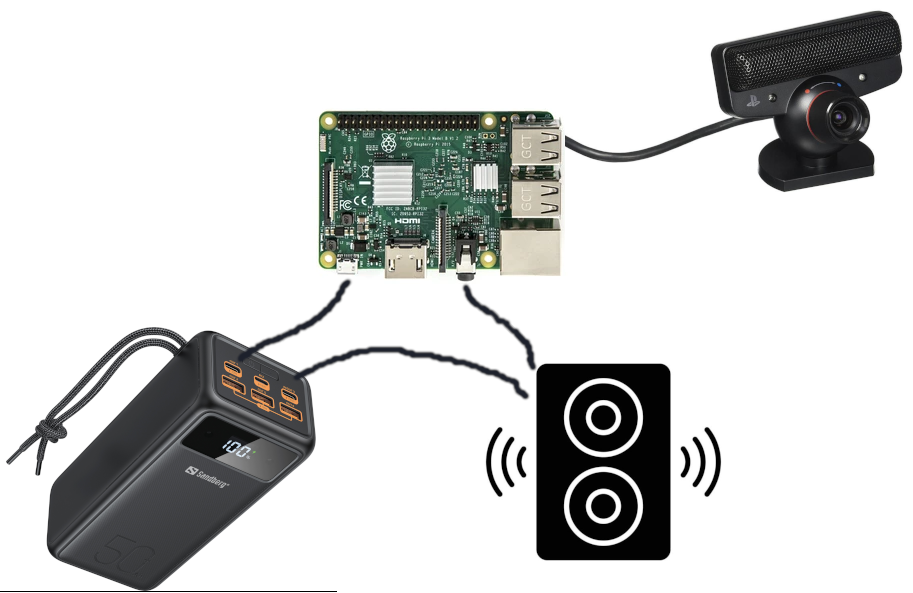
\includegraphics[width=0.7\linewidth]{schema.png}
	     \caption{Setup hardware completo alimentato da powerbank USB.}
	     \label{fig:hardware}
	 \end{figure}

Tutto l’hardware può essere gestito da remoto tramite accesso SSH per la shell e SFTP per lo scambio di file, permettendo aggiornamenti e manutenzione rapidi.

% --- Sottosezione Software ---

\subsection{Architettura Software}
\label{sec:software}

Il software principale è sviluppato in Python e organizzato in diversi moduli chiave.

\subsubsection{Monitoraggio Audio e Attivazione Eco}

Lo script centrale, \texttt{audio\_monitor\_echo\_service.py}, registra continuamente l’audio dal microfono USB, calcola i valori RMS e dBFS e attiva l’effetto eco se il volume supera la soglia configurata.  
Espone inoltre una API REST locale per l’interazione in tempo reale.

\textbf{Estratto di codice significativo:}
\begin{lstlisting}[language=Python]
	# Ciclo di monitoraggio
	def monitor_thread():
	global current_volume, mic_enabled
	while True:
	if mic_enabled:
	audio = sd.rec(int(FRAME_DURATION * SAMPLE_RATE),
	samplerate=SAMPLE_RATE, channels=CHANNELS, dtype='int16')
	sd.wait()
	arr = audio.astype(np.float32)
	rms = np.sqrt(np.mean(arr**2))
	dbfs = rms_to_dbfs(rms)
	if dbfs > THRESHOLD_DBFS:
	log(f"Superata soglia! dbfs={dbfs:.1f}. Attivo eco...")
	trigger_echo(arr.flatten())
\end{lstlisting}

\subsubsection{Effetto Eco: Simulazione del Delay a Nastro}

L’algoritmo di eco simula il classico delay a nastro: il frame audio registrato viene riprodotto con tap (ripetizioni) configurabili, ritardo, feedback e fading del volume.

\begin{lstlisting}[language=Python]
	def create_echo_buffer(audio, taps, delay_sec, feedback, start_vol, end_vol):
	n_samples = len(audio)
	delay_samples = int(delay_sec * SAMPLE_RATE)
	envelope = np.linspace(start_vol, end_vol, taps)
	out = np.zeros(n_samples + delay_samples * taps, dtype=np.float32)
	out[:n_samples] += audio.flatten()
	for i in range(taps):
	start = delay_samples * (i + 1)
	end = start + n_samples
	if end > len(out): break
	echo = audio.flatten() * envelope[i]
	if feedback > 0 and i > 0:
	echo += out[start-delay_samples:end-delay_samples] * feedback
	out[start:end] += echo
	return out
\end{lstlisting}

Parametri come ritardo, tap, feedback e fading sono regolabili dalla dashboard (vedi sottosezione dashboard).  
Questa implementazione riprende il comportamento delle unità echo vintage a nastro, dove tempo di delay, feedback e livelli di uscita erano fondamentali.

\subsubsection{Avvio Automatico del Servizio}

Lo script di monitoraggio viene avviato automaticamente all’accensione tramite un servizio systemd.  
\textbf{Esempio di unit file systemd:}

\begin{lstlisting}[language=bash]
	[Unit]
	Description=Audio Monitor & Echo Service
	After=network.target sound.target
	
	[Service]
	Type=simple
	User=rombo
	ExecStart=/home/rombo/00_APPLICATION/start_audio_monitor.sh
	WorkingDirectory=/home/rombo/00_APPLICATION
	Restart=on-failure
	
	[Install]
	WantedBy=multi-user.target
\end{lstlisting}

Qualsiasi aggiornamento agli script Python o ai file di configurazione può essere effettuato da remoto via SSH/SFTP e attivato riavviando il servizio.

\subsubsection{API REST e Configurazione}

Il servizio audio espone endpoint REST per la lettura del volume, la modifica delle soglie e la gestione dei parametri dell’eco:

\begin{itemize}
	\item \texttt{/volume} — Livello di rumore attuale (RMS, dBFS)
	\item \texttt{/threshold} — Leggi/imposta la soglia
	\item \texttt{/echo\_params} — Leggi/imposta parametri eco
	\item \texttt{/lockout} — Leggi/imposta tempo di lockout
	\item \texttt{/status} — Stato completo del sistema
	\item \texttt{/start\_echo} — Avvio manuale dell’eco
\end{itemize}

La configurazione è persistente tramite \texttt{threshold\_config.json}.

% --- Sottosezione Dashboard ---

\subsection{Dashboard e Controllo Real-Time}
\label{sec:dashboard}

La dashboard web, accessibile tramite l’IP statico del Raspberry Pi (protetta da Nginx e password hardcoded), offre controllo completo e visualizzazione in tempo reale del sistema.

\subsubsection{Funzionalità Principali}

\begin{figure}[ht]
	\centering
	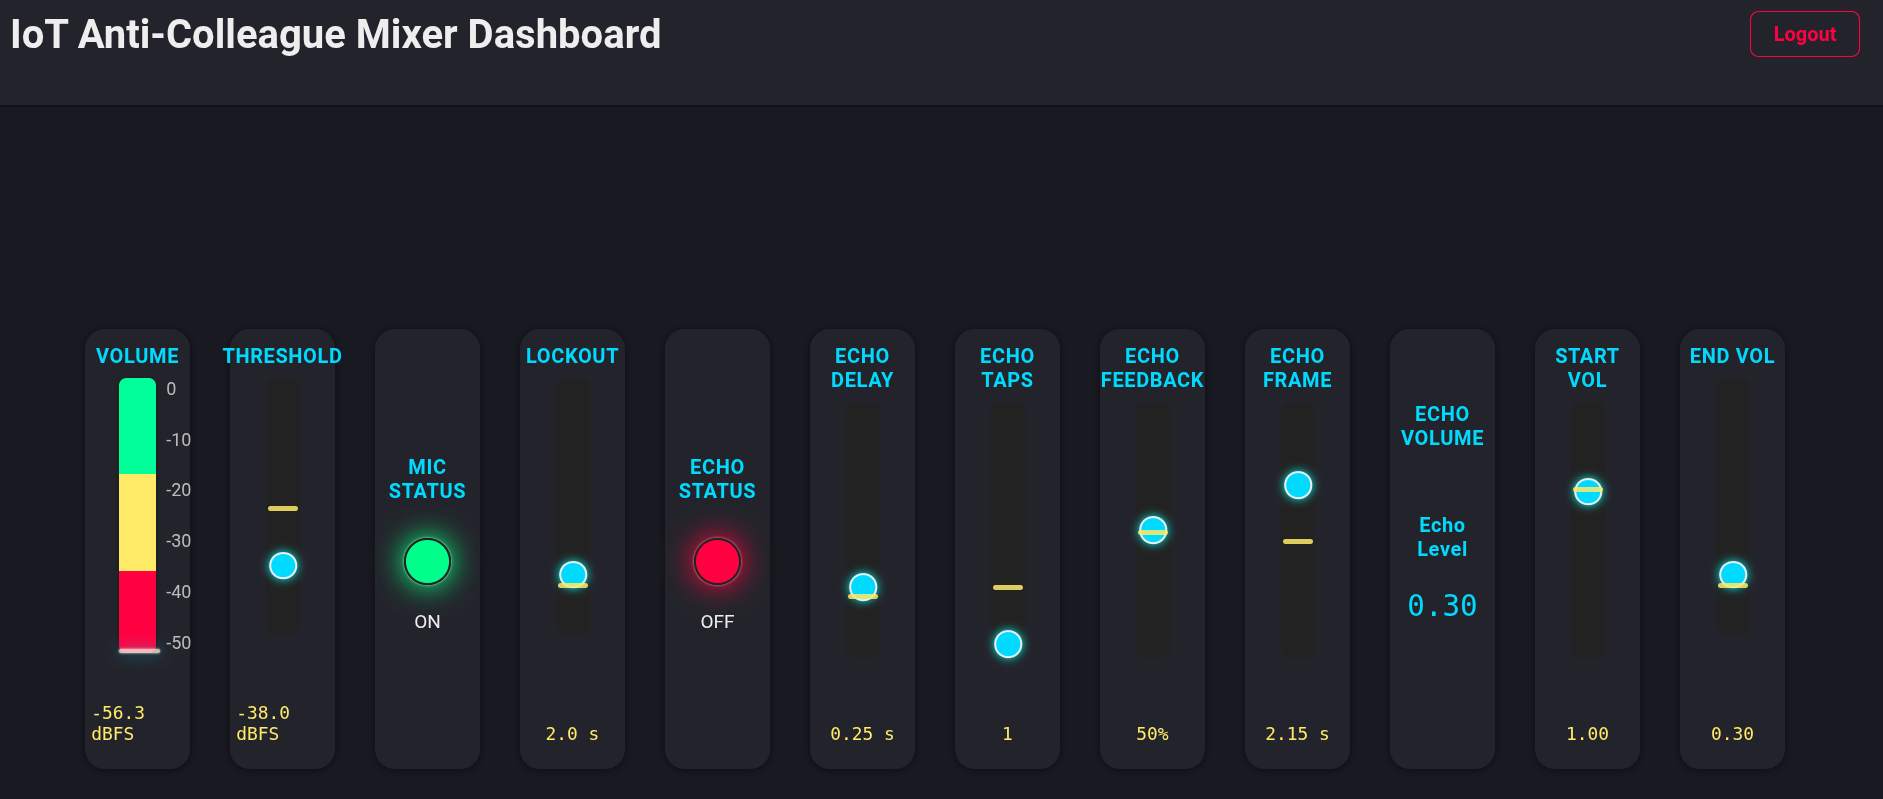
\includegraphics[width=0.9\linewidth]{mixer.png}
	\caption{Dashboard web.}
	\label{fig:dashboard}
\end{figure}

\begin{itemize}
	\item \textbf{Vmeter:} Visualizzazione live del dBFS rilevato dal microfono.
	\item \textbf{Slider:} Regolazione soglia, lockout, delay eco, tap, feedback, volume iniziale/finale e durata frame.
	\item \textbf{Lampade di stato:} Indicazione di attività microfono ed eco.
	\item \textbf{Animazione eco:} Visualizzazione live del “livello eco” durante la riproduzione.
\end{itemize}

\subsubsection{Aggiornamento Real-Time}

La dashboard JavaScript (\texttt{mixer.js}) interroga l’API REST backend ogni 200ms e aggiorna istantaneamente tutti i controlli e indicatori.

\begin{lstlisting}[language=JavaScript]
	// Poll dello stato e aggiornamento UI
	async function pollStatus() {
		const resp = await fetch("/api/status");
		const data = await resp.json();
		// Aggiorna Vmeter, slider, lampade, timer, ecc.
	}
	setInterval(pollStatus, 200);
\end{lstlisting}

L’accesso alla dashboard è protetto da Nginx come reverse proxy e da una password (memorizzata in \texttt{password.json} e verificata nel frontend Flask).

% --- Sottosezione Cloud ---

\subsection{Log degli Eventi e Analisi Cloud}

Ogni volta che l’eco viene attivato automaticamente (superamento soglia), un evento viene registrato sia localmente (CSV) che su ThingSpeak cloud:

\subsubsection{Registrazione e Invio Dati}

\begin{itemize}
	\item \textbf{Log CSV:} \texttt{event\_log.csv} contiene timestamp e dBFS per ogni evento.
	\item \textbf{ThingSpeak:} Gli eventi sono inviati via HTTP REST API usando le credenziali in \texttt{config.json}.
\end{itemize}

\begin{lstlisting}[language=Python]
	def log_event_thingspeak(dbfs, ts_iso):
	payload = {
		"api_key": write_api_key,
		"field1": dbfs,
		"field2": ts_iso,
	}
	url = "https://api.thingspeak.com/update.json"
	requests.post(url, data=payload, timeout=6)
\end{lstlisting}

La dashboard ThingSpeak fornisce grafici storici e statistiche sugli eventi di rumore, essenziali per comprendere i pattern e migliorare l’ergonomia dell’ambiente di lavoro.

% --- Sottosezione Esperienza Reale ---

\subsection{Deployment e Impatto}

Il sistema è stato installato in uno spazio co-working e ha immediatamente ridotto comportamenti rumorosi e urla (soprattutto telefonate e esclamazioni ad alto volume), rendendo l’ambiente sensibilmente più tranquillo e produttivo.

% --- Inserisci qui foto/testimonianza d’uso ---
% \begin{figure}[ht]
	%     \centering
	%     \includegraphics[width=0.7\linewidth]{office_usage.jpg}
	%     \caption{Dispositivo in azione in un vero ambiente di co-working.}
	%     \label{fig:usage}
	% \end{figure}

%------------------------------------------------

\section{Risultati}

\subsection{Risultati della sperimentazione}

\subsubsection{Analisi dei dati raccolti}

Durante le due settimane di sperimentazione, il dispositivo è stato installato al centro dell'ufficio, alimentato tramite powerbank USB (ricaricato ogni sera). L'approccio iniziale era giocoso, ma ben presto il sistema ha stimolato una riflessione collettiva sul comportamento in open space, risultando non invasivo e accettato dalla maggior parte dei colleghi.

I parametri impostati tramite la dashboard web sono rimasti pressoché invariati per tutto il periodo, grazie a una taratura efficace fin dalla prima installazione.

\paragraph{Grafico 1: Volume dei trigger nel tempo}

Il primo grafico mostra l'andamento del livello di volume \texttt{noise\_dbfs} che ha causato il trigger dell'eco, in funzione del tempo.

\begin{figure}[h!]
	\centering
	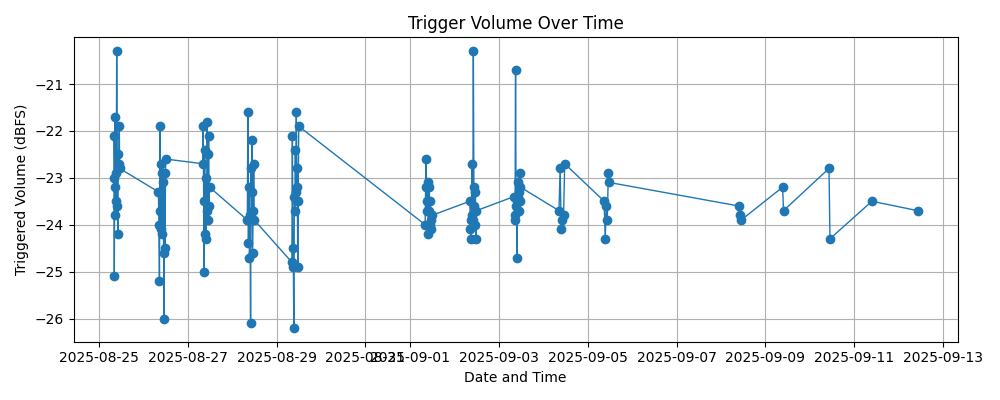
\includegraphics[width=0.92\linewidth]{trigger_volume_vs_time.png}
	\caption{Livello di volume (dBFS) degli eventi di trigger nel tempo.}
	\label{fig:trigger_volume_time}
\end{figure}

Come si osserva, il livello di volume che ha causato l'attivazione dell'eco è rimasto pressoché costante, a conferma che il comportamento indesiderato era sempre riconducibile a superamenti netti della soglia impostata.

\paragraph{Grafico 2: Numero di trigger giornalieri}

Il secondo grafico mostra il numero di attivazioni giornaliere del sistema.

\begin{figure}[h!]
	\centering
	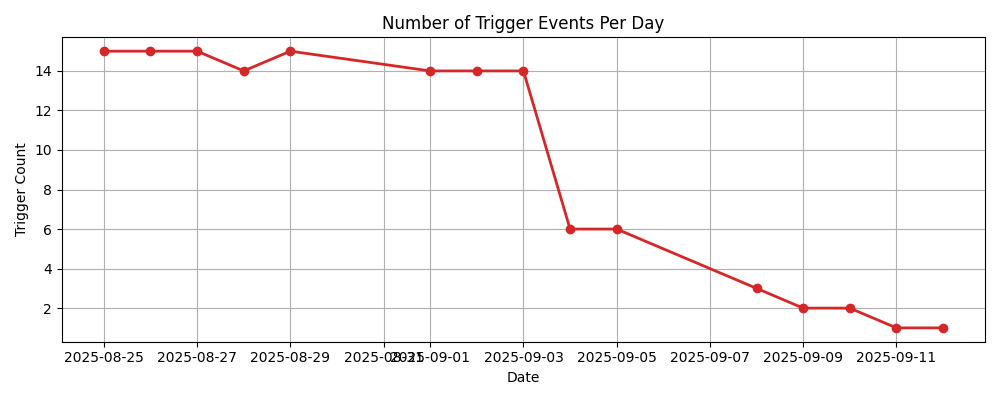
\includegraphics[width=0.92\linewidth]{trigger_count_per_day.png}
	\caption{Numero di eventi di trigger registrati per ciascun giorno lavorativo.}
	\label{fig:trigger_count_day}
\end{figure}

Questo grafico evidenzia chiaramente il trend discendente degli episodi di disturbo: nei primi giorni il numero di trigger era elevato, ma progressivamente si è ridotto fino a stabilizzarsi su minimi fisiologici, segno che i colleghi hanno interiorizzato la necessità di mantenere un comportamento più rispettoso.

\subsubsection{Considerazioni sull'impatto sociale e ambientale}

L'esperienza in ufficio ha mostrato come la semplice presenza del dispositivo abbia sensibilizzato la maggior parte dei colleghi a tenere un tono di voce più consono e a spostarsi nella sala comune per rispondere alle telefonate. Su otto colleghi, solo uno ha manifestato una certa avversione percependo il sistema come un controllo invasivo, ma il clima generale è rapidamente migliorato e si è consolidato un comportamento più attento al benessere collettivo.

La sperimentazione, durata \textbf{due settimane lavorative} (escludendo sabato e domenica), ha raggiunto pienamente l'obiettivo del progetto: non solo ridurre i picchi di rumore, ma soprattutto favorire una cultura della collaborazione e del rispetto nei luoghi di lavoro condivisi.

\subsubsection{Conclusioni operative}

I dati raccolti e i grafici presentati dimostrano che l'approccio tecnologico, se ben calibrato e comunicato, può essere uno strumento efficace per la gestione del benessere in open space, favorendo l'autoregolazione e la consapevolezza dei comportamenti.


\section{Conclusioni}


L'esperimento condotto con il dispositivo IoT anti-collega rumoroso ha raggiunto pienamente il suo obiettivo: mitigare in modo efficace il problema del rumore eccessivo negli ambienti di lavoro condivisi. Fin dalla sua installazione, il sistema ha favorito una maggiore consapevolezza nei comportamenti dei colleghi, portando a un netto miglioramento del clima generale in ufficio e alla riduzione degli episodi di disturbo. \newline

Tuttavia, come emerso durante la sperimentazione, una soluzione di questo tipo non può essere adottata in modo continuativo e permanente. La presenza costante dell'eco sonoro, seppur utile in fase iniziale per sensibilizzare e correggere le cattive abitudini, rischia a lungo andare di generare un senso di oppressione e controllo eccessivo. Questo aspetto è stato confermato dal feedback dei partecipanti, che hanno apprezzato l'efficacia del sistema ma hanno sottolineato l'importanza di un approccio equilibrato e non invasivo. \newline

Qui emerge la vera forza dell'IoT e della raccolta dati automatizzata: grazie alla piattaforma online e al monitoraggio continuo, il datore di lavoro può scegliere di mantenere attivo il sistema in modalità "passiva", con gli altoparlanti spenti ma con la raccolta dati sempre attiva. In questo modo, è possibile tenere sotto controllo l'ambiente lavorativo senza intervenire direttamente, analizzando i trend e rilevando eventuali peggioramenti nel comportamento acustico. Solo in caso di necessità, e dopo aver affrontato la questione con i dipendenti, si può valutare di riattivare l'eco come strumento di deterrenza. \newline

Per quanto riguarda gli sviluppi futuri, il progetto può essere ulteriormente ottimizzato sia in termini di consumi energetici che di ingombro, integrando soluzioni hardware più compatte e algoritmi di gestione più efficienti. Tuttavia, dal punto di vista operativo, la sperimentazione ha dimostrato che già l'attuale sistema svolge egregiamente il proprio lavoro, rappresentando un valido esempio di applicazione intelligente delle tecnologie IoT per il benessere negli ambienti di lavoro. \newline

%----------------------------------------------------------------------------------------
%	REFERENCE LIST
%----------------------------------------------------------------------------------------

\phantomsection
\bibliographystyle{unsrt}
\bibliography{sample.bib}

%----------------------------------------------------------------------------------------

\end{document}
